\chapter{ความสัมพันธ์และฟังก์ชัน (Relations and Functions)}
\label{ch:relations}
\label{sec:relation-intro}

ฟังก์ชันและความสัมพันธ์เป็นแนวคิดพื้นฐานทางคณิตศาสตร์ที่ใช้อธิบายโครงสร้างข้อมูล การส่งผ่านค่า และการกำหนดกติกาในการประมวลผลของระบบคอมพิวเตอร์ ในการเขียนโปรแกรม ฟังก์ชันทำหน้าที่รับข้อมูลเข้าประมวลผลตามเงื่อนไข แล้วส่งผลลัพธ์กลับออกมาเพียงค่าเดียวสำหรับข้อมูลเข้าแต่ละชุด ขณะที่ความสัมพันธ์มีเงื่อนไขผ่อนคลายกว่า จึงใช้อธิบายการเชื่อมโยงแบบหลายต่อหลายได้ เช่น การเชื่อมโยงระหว่างตารางในฐานข้อมูล หรือการเชื่อมโยงระหว่างโหนดในกราฟ

บทนี้เริ่มจากคู่อันดับและผลคูณคาร์ทีเซียนซึ่งเป็นรากฐานของความสัมพันธ์ ต่อด้วยคุณสมบัติของความสัมพันธ์ทวิภาคและการปิดคุณสมบัติ จากนั้นจึงพัฒนาเข้าสู่ฟังก์ชันซึ่งเป็นความสัมพันธ์ชนิดพิเศษ และปิดท้ายด้วยลำดับและอนุกรมซึ่งเป็นฟังก์ชันที่มีโดเมนเป็นจำนวนเต็มบวก พร้อมการประยุกต์ใช้ในงานฐานข้อมูล การวิเคราะห์อัลกอริทึม และโครงสร้างข้อมูลตารางแฮช

\section{พื้นฐานความสัมพันธ์และคู่อันดับ}
\label{sec:basic-relation}

แนวคิดเรื่องคู่อันดับและความสัมพันธ์เป็นรากฐานสำคัญในการกำหนดโครงสร้างการจับคู่สมาชิกจากเซตหนึ่งไปยังอีกเซตหนึ่ง คู่อันดับ $(a,b)$ ทำหน้าที่ระบุทิศทางที่แน่นอนระหว่างสมาชิก $a \in A$ และ $b \in B$ โดยลำดับมีผลต่อความหมาย ขณะที่ความสัมพันธ์ $R \subseteq A \times B$ คือเซตย่อยของผลคูณคาร์ทีเซียนที่รวบรวมการจับคู่ตามเงื่อนไขทางคณิตศาสตร์ เพื่อนำไปใช้เป็นแบบจำลองโครงสร้างข้อมูลและแบบจำลองฐานข้อมูลเชิงสัมพันธ์

แนวคิดเรื่องความสัมพันธ์มีรากฐานมาจากทฤษฎีเซตที่เกออร์ก คันทอร์ (Georg Cantor) พัฒนาขึ้นในช่วงปลายศตวรรษที่ 19~\cite{halmos1974naive} ต่อมาในผลงาน Principia Mathematica ซึ่งเผยแพร่ในปี ค.ศ. 1910 อัลเฟรด นอร์ธ วิทเฮด (Alfred North Whitehead) และเบอร์ทรันด์ รัสเซลล์ (Bertrand Russell) ได้ผนวกแนวคิดความสัมพันธ์เข้ากับตรรกศาสตร์สัญลักษณ์ โดยนิยามความสัมพันธ์ในรูปเซตของคู่อันดับ~\cite{russell1910principia} ในสาขาวิทยาการคอมพิวเตอร์ เอ็ดการ์ คอดด์ (Edgar F. Codd) ได้นำทฤษฎีความสัมพันธ์มาสร้างแบบจำลองฐานข้อมูลเชิงสัมพันธ์ (Relational Model) ในปี ค.ศ. 1970 ซึ่งกลายเป็นรากฐานของระบบฐานข้อมูลในปัจจุบัน~\cite{codd1970relational}

คู่อันดับ (Ordered Pair) เป็นโครงสร้างพื้นฐานในการระบุทิศทางการจับคู่ โดยคู่อันดับ $(a,b)$ จะแตกต่างจากเซตตรงที่ลำดับมีผลต่อความหมาย กล่าวคือ $(a,b) \neq (b,a)$ เมื่อ $a \neq b$ ผลคูณคาร์ทีเซียน (Cartesian Product) ของเซต $A$ และ $B$ เขียนแทนด้วย $A \times B$ คือเซตของคู่อันดับทั้งหมด $(a,b)$ โดยที่ $a \in A$ และ $b \in B$ ดังที่ได้ศึกษาใน~\autoref{sec:cartesian-product}

\begin{definition}[ความสัมพันธ์]
\index{ความสัมพันธ์!นิยาม}
ให้ $A$ และ $B$ เป็นเซตใดๆ ความสัมพันธ์ (Relation) จาก $A$ ไปยัง $B$ คือเซตย่อยของผลคูณคาร์ทีเซียน $A \times B$ นั่นคือ $R \subseteq A \times B$

หาก $(a,b) \in R$ จะเขียนแทนด้วย $a\,R\,b$ หมายถึง ``$a$ มีความสัมพันธ์กับ $b$ โดย $R$''  
หาก $(a,b) \notin R$ จะเขียนแทนด้วย $a\,\centernot{R}\,b$ หมายถึง ``$a$ ไม่มีความสัมพันธ์กับ $b$ โดย $R$''
\end{definition}

\begin{ex}
\label{ex:total-relations-count}
กำหนดให้ $A = \{1, 2, 3\}$ และ $B = \{x, y\}$ จงหาสิ่งต่อไปนี้
\begin{enumerate}[label=\textbf{\arabic*.}]
    \item จำนวนสมาชิกของผลคูณคาร์ทีเซียน $|A \times B|$
    \item จำนวนความสัมพันธ์ทั้งหมดที่เป็นไปได้จาก $A$ ไป $B$
    \item จำนวนความสัมพันธ์ทวิภาคทั้งหมดที่เป็นไปได้บนเซต $A$
\end{enumerate}
\end{ex}
\begin{solution}
\begin{enumerate}[label=\textbf{\arabic*.}]
    \item จากสูตรผลคูณคาร์ทีเซียน $|A \times B| = |A| \times |B| = 3 \times 2 = 6$
    \item ความสัมพันธ์จาก $A$ ไป $B$ คือเซตย่อยใดๆ ของ $A \times B$ ดังนั้นจำนวนความสัมพันธ์ทั้งหมดเท่ากับจำนวนเพาเวอร์เซต $|\mathcal{P}(A \times B)| = 2^{|A \times B|} = 2^6 = 64$ ความสัมพันธ์
    \item ความสัมพันธ์ทวิภาคบน $A$ คือเซตย่อยของ $A \times A$ โดยมีสมาชิก $|A \times A| = 3 \times 3 = 9$ ดังนั้นจำนวนความสัมพันธ์ทวิภาคบน $A$ เท่ากับ $2^{|A|^2} = 2^9 = 512$ ความสัมพันธ์
\end{enumerate}
\end{solution}

\begin{ex}
\label{ex:relation-operations}
กำหนด $A = \{1, 2, 3\}$ และ $B = \{a, b\}$ โดยมีความสัมพันธ์ $R_1 = \{(1,a), (2,b), (3,a)\}$ และ $R_2 = \{(1,b), (2,b), (3,a)\}$ จาก $A$ ไป $B$ จงหาการดำเนินการต่อไปนี้
\begin{enumerate}[label=\textbf{\arabic*.}]
    \item การยูเนียน $R_1 \cup R_2$
    \item การอินเตอร์เซกชัน $R_1 \cap R_2$
    \item ผลต่าง $R_1 - R_2$
    \item คอมพลีเมนต์ $\overline{R_1}$ เทียบกับเอกภพสัมพัทธ์ $A \times B$
\end{enumerate}
\end{ex}
\begin{solution}
\begin{enumerate}[label=\textbf{\arabic*.}]
    \item $R_1 \cup R_2 = \{(1,a), (1,b), (2,b), (3,a)\}$
    \item $R_1 \cap R_2 = \{(2,b), (3,a)\}$
    \item $R_1 - R_2 = \{(1,a)\}$
    \item เนื่องจาก $A \times B = \{(1,a),(1,b),(2,a),(2,b),(3,a),(3,b)\}$ จะได้ว่า
    \[ \overline{R_1} = (A \times B) - R_1 = \{(1,b), (2,a), (3,b)\} \]
\end{enumerate}
\solhere
\end{solution}

นอกจากการเขียนความสัมพันธ์ในรูปเซตของคู่อันดับแล้ว ความสัมพันธ์บนเซตจำกัดยังเขียนแทนได้ด้วยตารางค่าศูนย์และหนึ่งที่เรียกว่าเมทริกซ์บูลีน (Boolean Matrix) ซึ่งเป็นรูปแบบที่เครื่องคอมพิวเตอร์จัดเก็บและประมวลผลได้โดยตรง หลักการคือกำหนดให้แถวที่ $i$ แทนสมาชิกตัวที่ $i$ ของเซตต้นทาง และคอลัมน์ที่ $j$ แทนสมาชิกตัวที่ $j$ ของเซตปลายทาง แล้วกำหนดค่าในช่อง $(i,j)$ เป็น $1$ เมื่อสมาชิกทั้งสองมีความสัมพันธ์กัน และเป็น $0$ เมื่อไม่มีความสัมพันธ์กัน

\begin{ex}
\label{ex:matrix-relation-rep}
กำหนด $A = \{1, 2, 3, 4\}$ และความสัมพันธ์ $R = \{(x,y) \in A \times A \mid x \text{ หาร } y \text{ ลงตัว}\}$ จงเขียนเซตสมาชิกของความสัมพันธ์ $R$ และเขียนเมทริกซ์บูลีน $M_R$
\end{ex}
\begin{solution}
พิจารณาการหารลงตัวของสมาชิกใน $A$ จะได้
\begin{align*}
1 \text{ หาร } 1, 2, 3, 4 \text{ ลงตัว} &\implies (1,1), (1,2), (1,3), (1,4) \in R\\
2 \text{ หาร } 2, 4 \text{ ลงตัว} &\implies (2,2), (2,4) \in R\\
3 \text{ หาร } 3 \text{ ลงตัว} &\implies (3,3) \in R\\
4 \text{ หาร } 4 \text{ ลงตัว} &\implies (4,4) \in R
\end{align*}
จะได้ $R = \{(1,1),(1,2),(1,3),(1,4),(2,2),(2,4),(3,3),(4,4)\}$ และเขียนเป็นเมทริกซ์บูลีนขนาด $4 \times 4$ ได้ดังนี้
\[ M_R = \begin{bmatrix} 1 & 1 & 1 & 1 \\ 0 & 1 & 0 & 1 \\ 0 & 0 & 1 & 0 \\ 0 & 0 & 0 & 1 \end{bmatrix} \]
\solhere
\end{solution}

\subsection{โดเมน เรนจ์ และความสัมพันธ์ผกผัน}
ในระบบลงทะเบียนเรียน ความสัมพันธ์ระหว่างนักศึกษากับรายวิชาไม่จำเป็นต้องครอบคลุมนักศึกษาทุกคน เพราะบางคนอาจยังไม่ได้ลงทะเบียน และไม่จำเป็นต้องครอบคลุมทุกรายวิชา เพราะบางวิชาอาจยังไม่มีผู้ลงทะเบียน เซตของนักศึกษาที่ปรากฏจริงในรายการลงทะเบียนเรียกว่าโดเมนของความสัมพันธ์ ส่วนเซตของรายวิชาที่มีผู้ลงทะเบียนจริงเรียกว่าเรนจ์ของความสัมพันธ์ และเมื่อกลับทิศทางการมองจากรายวิชาย้อนไปหานักศึกษาผู้ลงทะเบียน จะได้ความสัมพันธ์ใหม่ที่เรียกว่าความสัมพันธ์ผกผัน ซึ่งเกิดจากการสลับตำแหน่งสมาชิกในคู่อันดับทุกคู่

\begin{definition}[โดเมน เรนจ์ และความสัมพันธ์ผกผัน]
\index{ความสัมพันธ์!โดเมน}
\index{ความสัมพันธ์!เรนจ์}
\index{ความสัมพันธ์!ผกผัน}
ให้ $R$ เป็นความสัมพันธ์จากเซต $A$ ไปยังเซต $B$
\begin{enumerate}[label=\textbf{\arabic*.}]
    \item โดเมน (Domain) ของ $R$ คือ $\mathcal{D}(R) = \{a \in A \mid \exists b \in B,\ (a,b) \in R\}$
    \item เรนจ์ (Range) ของ $R$ คือ $\mathcal{R}(R) = \{b \in B \mid \exists a \in A,\ (a,b) \in R\}$
    \item ความสัมพันธ์ผกผัน (Inverse Relation) ของ $R$ คือ $R^{-1} = \{(b,a) \mid (a,b) \in R\} \subseteq B \times A$
\end{enumerate}
\end{definition}

โดเมนเป็นเซตย่อยของ $A$ และเรนจ์เป็นเซตย่อยของ $B$ เสมอ แต่ไม่จำเป็นต้องเท่ากับเซตต้นทางและเซตปลายทาง สมาชิกใน $A$ ที่ไม่ปรากฏในตำแหน่งแรกของคู่อันดับใดเลยจะไม่อยู่ในโดเมน และสมาชิกใน $B$ ที่ไม่ปรากฏในตำแหน่งที่สองของคู่อันดับใดเลยจะไม่อยู่ในเรนจ์ ส่วนความสัมพันธ์ผกผันมีสมบัติที่ตรวจสอบได้โดยตรงจากนิยาม ได้แก่ $\mathcal{D}(R^{-1}) = \mathcal{R}(R)$, $\mathcal{R}(R^{-1}) = \mathcal{D}(R)$ และการผกผันซ้ำสองครั้งจะได้ความสัมพันธ์เดิม นั่นคือ $(R^{-1})^{-1} = R$

\begin{ex}
\label{ex:domain-range-inverse}
กำหนด $A = \{1,2,3,4\}$, $B = \{a,b,c\}$ และความสัมพันธ์ $R = \{(1,a),(1,b),(2,b),(4,a)\}$ จาก $A$ ไป $B$ จงหาโดเมน เรนจ์ และความสัมพันธ์ผกผันของ $R$
\end{ex}
\begin{solution}
\begin{align*}
\mathcal{D}(R) &= \{1,2,4\} \quad (3 \text{ ไม่ปรากฏในตำแหน่งแรกของคู่อันดับใดเลย})\\
\mathcal{R}(R) &= \{a,b\} \quad (c \text{ ไม่ปรากฏในตำแหน่งที่สองของคู่อันดับใดเลย})\\
R^{-1} &= \{(a,1),(b,1),(b,2),(a,4)\}
\end{align*}
$\therefore \mathcal{D}(R) = \{1,2,4\}$, $\mathcal{R}(R) = \{a,b\}$ และ $R^{-1} = \{(a,1),(b,1),(b,2),(a,4)\}$ \solhere
\end{solution}

\section{คุณสมบัติและการขยายความสัมพันธ์}
\label{sec:relation-properties}

ความสัมพันธ์ที่นิยามบนเซตเดียวกัน นั่นคือ $R \subseteq A \times A$ เรียกว่าความสัมพันธ์ทวิภาค (Binary Relation on a Set) ซึ่งเป็นรูปแบบที่พบมากที่สุดในงานคอมพิวเตอร์ เพราะใช้อธิบายการเชื่อมโยงระหว่างสิ่งของชนิดเดียวกัน เช่น การเชื่อมโยงระหว่างหน้าเว็บด้วยไฮเปอร์ลิงก์ การเชื่อมโยงระหว่างผู้ใช้ในเครือข่ายสังคม หรือการเชื่อมโยงระหว่างคำสั่งที่ต้องทำงานตามลำดับก่อนหลัง หัวข้อนี้ศึกษาคุณสมบัติพื้นฐานสี่ประการที่ใช้จำแนกความสัมพันธ์ทวิภาค การประกอบความสัมพันธ์เพื่อหาเส้นทางหลายขั้น และการปิดคุณสมบัติซึ่งเป็นการเติมคู่อันดับเพิ่มให้ความสัมพันธ์มีคุณสมบัติที่ต้องการ

\subsection{คุณสมบัติพื้นฐาน 4 ประการ}
การวิเคราะห์โครงสร้างความสัมพันธ์ทวิภาค $R \subseteq A \times A$ อาศัยการตรวจสอบพฤติกรรมการจับคู่ของสมาชิกในเซตเดียวกัน ความสัมพันธ์ที่มีรูปแบบแน่นอนจะสอดคล้องกับคุณสมบัติทางคณิตศาสตร์ 4 ประการ ได้แก่ สะท้อน สมมาตร ปฏิสมมาตร และถ่ายทอด ความสัมพันธ์หนึ่งอาจมีคุณสมบัติเหล่านี้พร้อมกันหลายข้อ ไม่มีข้อใด หรือมีเพียงบางข้อ การระบุว่าความสัมพันธ์ใดมีคุณสมบัติใดบ้างจึงเป็นขั้นตอนแรกของการวิเคราะห์โครงสร้างข้อมูลที่ใช้ความสัมพันธ์นั้นเป็นแบบจำลอง

\begin{definition}[คุณสมบัติของความสัมพันธ์ทวิภาค]
\index{ความสัมพันธ์!คุณสมบัติ}
ให้ $R$ เป็นความสัมพันธ์บนเซต $A$
\begin{enumerate}[label=\textbf{\arabic*.}]
    \item การสะท้อน (Reflexive) คือ สำหรับทุก $a \in A$ จะได้ $(a, a) \in R$
    \item การสมมาตร (Symmetric) คือ ถ้า $(a, b) \in R$ แล้ว $(b, a) \in R$
    \item ความเป็นปฏิสมมาตร (Antisymmetric) คือ ถ้า $(a, b) \in R$ และ $(b, a) \in R$ แล้ว $a = b$
    \item การถ่ายทอด (Transitive) คือ ถ้า $(a, b) \in R$ และ $(b, c) \in R$ แล้ว $(a, c) \in R$
\end{enumerate}
\end{definition}

คุณสมบัติทั้งสี่ประการมีลักษณะเชิงโครงสร้างที่สังเกตได้จากแผนภาพลูกศร คุณสมบัติสะท้อนปรากฏเป็นลูกศรวนรอบตัวเองที่จุดทุกจุด คุณสมบัติสมมาตรปรากฏเป็นลูกศรสองทิศทางระหว่างจุดคู่หนึ่ง คุณสมบัติปฏิสมมาตรอนุญาตให้มีลูกศรเพียงทิศทางเดียวระหว่างจุดที่ต่างกัน และคุณสมบัติถ่ายทอดกำหนดว่าเมื่อเดินจากจุดหนึ่งไปยังอีกจุดหนึ่งได้สองขั้น จะต้องมีลูกศรตรงเชื่อมถึงกันด้วย ดังแสดงใน~\autoref{fig:relation-properties-thai}

\begin{figure}[H]
    \centering
    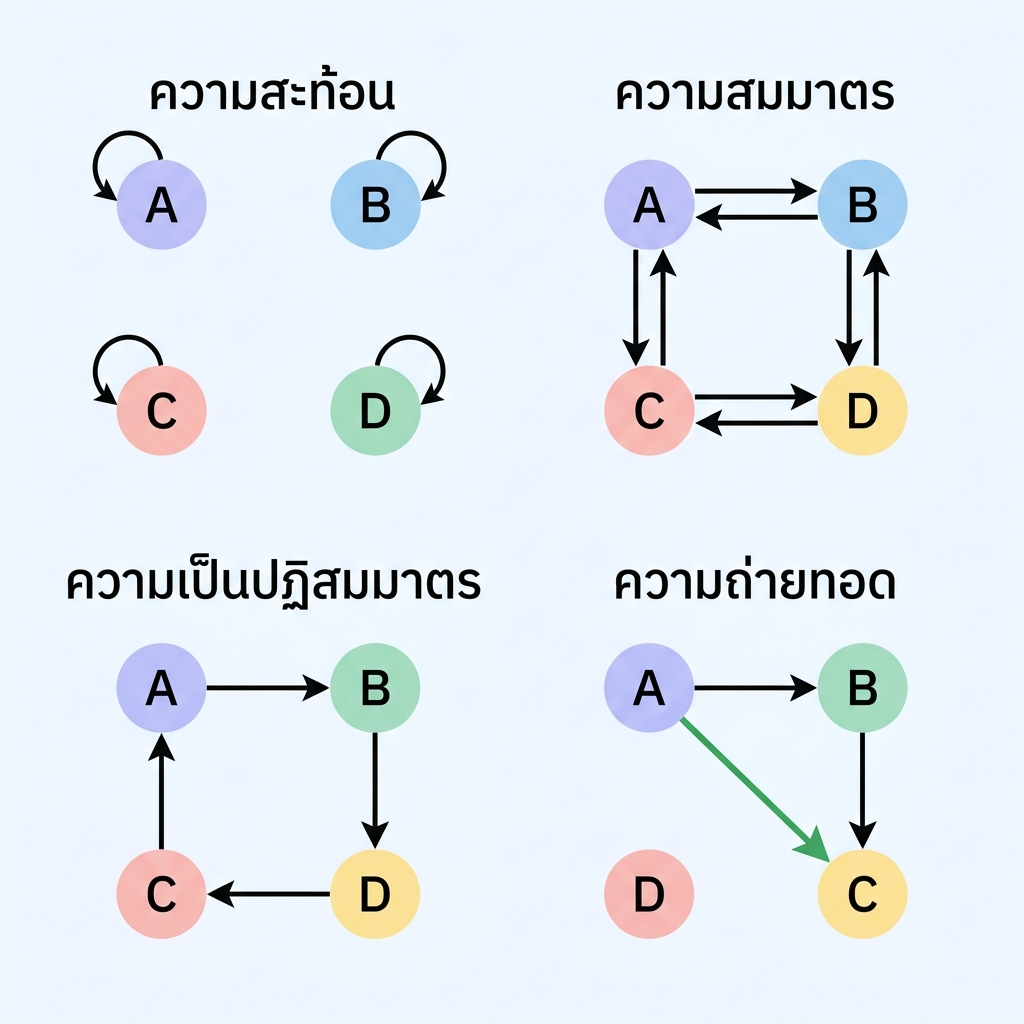
\includegraphics[width=0.68\textwidth]{Figures/png_ready/relation-properties-thai.png}
    \caption{คุณสมบัติ 4 ประการของความสัมพันธ์ทวิภาค}
    \label{fig:relation-properties-thai}
\end{figure}

\begin{ex}
\label{ex:relation-properties-check}
กำหนด $A = \{1, 2, 3\}$ และ $R_1 = \{(1,1), (2,2), (3,3), (1,2), (2,1)\}$ จงพิจารณาคุณสมบัติทั้ง 4 ประการ
\end{ex}
\begin{solution}
\begin{align*}
\text{สะท้อน} &\quad (1,1),(2,2),(3,3) \in R_1 \text{ ครบทุก } a \in A \Rightarrow \text{เป็นสะท้อน}\\
\text{สมมาตร} &\quad (1,2) \in R_1 \Rightarrow (2,1) \in R_1 \text{ และคู่ที่เหลือเป็นคู่ } (a,a) \Rightarrow \text{เป็นสมมาตร}\\
\text{ปฏิสมมาตร} &\quad (1,2),(2,1) \in R_1 \text{ แต่ } 1 \neq 2 \Rightarrow \text{ไม่เป็นปฏิสมมาตร}\\
\text{ถ่ายทอด} &\quad (1,2),(2,1) \Rightarrow (1,1) \in R_1 \text{ และ } (2,1),(1,2) \Rightarrow (2,2) \in R_1\\
&\quad \text{ส่วนคู่ที่เหลือมี } (a,a) \text{ เป็นสมาชิกหนึ่งจึงเป็นจริงเสมอ} \Rightarrow \text{เป็นถ่ายทอด}
\end{align*}
$\therefore R_1$ มีคุณสมบัติสะท้อน สมมาตร และถ่ายทอด แต่ไม่เป็นปฏิสมมาตร \solhere
\end{solution}

\subsection{การประกอบความสัมพันธ์}
ในระบบฐานข้อมูลบุคลากร ความสัมพันธ์ $R$ อาจเชื่อมพนักงานแต่ละคนเข้ากับแผนกที่สังกัด ขณะที่ความสัมพันธ์ $S$ เชื่อมแผนกเข้ากับอาคารที่ตั้งสำนักงาน การตอบคำถามว่าพนักงานคนหนึ่งทำงานอยู่ในอาคารใดจึงต้องเชื่อมความสัมพันธ์ทั้งสองเข้าด้วยกันโดยอาศัยแผนกเป็นตัวกลาง การเชื่อมต่อในลักษณะนี้เรียกว่าการประกอบความสัมพันธ์ ซึ่งเป็นเครื่องมือสำหรับหาเส้นทางที่มีความยาวหลายขั้นในกราฟ และเป็นพื้นฐานของการปิดถ่ายทอดในหัวข้อถัดไป

\begin{definition}[การประกอบความสัมพันธ์]
\index{ความสัมพันธ์!การประกอบ}
ให้ $R \subseteq A \times B$ และ $S \subseteq B \times C$ การประกอบความสัมพันธ์ (Composition of Relations) ของ $R$ กับ $S$ เขียนแทนด้วย $S \circ R \subseteq A \times C$ นิยามโดย
\[ S \circ R = \{(a,c) \in A \times C \mid \exists b \in B,\ (a,b) \in R \land (b,c) \in S\} \]
สำหรับความสัมพันธ์ $R$ บนเซต $A$ นิยามกำลังของความสัมพันธ์โดย $R^1 = R$ และ $R^{n+1} = R \circ R^n$ เมื่อ $n \ge 1$
\end{definition}

สัญลักษณ์ $S \circ R$ อ่านว่า ทำ $R$ ก่อนแล้วจึงทำ $S$ ซึ่งเป็นลำดับเดียวกับการประกอบฟังก์ชัน $g \circ f$ ที่จะศึกษาใน~\autoref{sec:functions} การตีความในเชิงกราฟคือ $(a,c) \in S \circ R$ ก็ต่อเมื่อมีเส้นทางเดินจาก $a$ ไปยัง $c$ โดยผ่านจุดกลาง $b$ เพียงจุดเดียว ดังนั้น $R^n$ จึงรวบรวมคู่ของจุดที่เดินถึงกันได้ด้วยเส้นทางความยาว $n$ ขั้นพอดี

\begin{ex}
\label{ex:relation-composition}
กำหนด $A = \{1,2,3\}$ และความสัมพันธ์ $R = \{(1,2),(2,3)\}$ บน $A$ จงหา $R^2$ และ $R^3$
\end{ex}
\begin{solution}
\begin{align*}
R^2 = R \circ R &= \{(a,c) \mid \exists b,\ (a,b) \in R \land (b,c) \in R\}\\
&= \{(1,3)\} \quad ((1,2) \in R \text{ และ } (2,3) \in R)\\
R^3 = R \circ R^2 &= \{(a,c) \mid \exists b,\ (a,b) \in R^2 \land (b,c) \in R\}\\
&= \varnothing \quad (\text{ไม่มีคู่อันดับใน } R \text{ ที่เริ่มต้นด้วย } 3)
\end{align*}
$\therefore R^2 = \{(1,3)\}$ และ $R^3 = \varnothing$ \solhere
\end{solution}

\subsection{การขยายและการปิดคุณสมบัติ}
ในการวิเคราะห์โครงสร้างความสัมพันธ์ ความสัมพันธ์เดิม $R$ อาจยังขาดคุณสมบัติบางประการที่จำเป็นต่อการประมวลผล การปิดคุณสมบัติ (Closure) เป็นกระบวนการขยายเซตความสัมพันธ์โดยเติมคู่อันดับเพิ่มเข้าไปใน $R$ ให้มีจำนวนน้อยที่สุด เพื่อสร้างความสัมพันธ์ใหม่ $R'$ ที่มีคุณสมบัติที่ต้องการอย่างสมบูรณ์ เช่น การปิดถ่ายทอด $t(R)$ ที่ใช้รวบรวมเส้นทางเชื่อมต่อทั้งหมดในทฤษฎีกราฟ โดยการปิดคุณสมบัติที่สำคัญ ได้แก่
\begin{enumerate}[label=\textbf{\arabic*.}]
    \item การปิดสะท้อน คือ $r(R) = R \cup \{(a,a) \mid a \in A\}$ ซึ่งเติมคู่อันดับที่จับคู่สมาชิกกับตัวเองให้ครบทุกตัว
    \item การปิดสมมาตร คือ $s(R) = R \cup R^{-1}$ ซึ่งเติมคู่อันดับทิศทางย้อนกลับให้ครบทุกคู่
    \item การปิดถ่ายทอด คือ $t(R) = R \cup R^2 \cup R^3 \cup \dots = \bigcup_{i=1}^{n} R^i$ ซึ่งรวบรวมเส้นทางเชื่อมต่อทุกความยาวเข้าไว้ด้วยกัน
\end{enumerate}

\begin{ex}
กำหนด $A = \{1, 2, 3\}$ และ $R = \{(1,2), (2,3)\}$ จงหา $r(R), s(R),$ และ $t(R)$
\end{ex}
\begin{solution}
\begin{align*}
r(R) &= R \cup \{(1,1), (2,2), (3,3)\} = \{(1,1),(2,2),(3,3),(1,2),(2,3)\}\\
s(R) &= R \cup R^{-1} = \{(1,2),(2,3),(2,1),(3,2)\}\\
t(R) &= R \cup R^2 = \{(1,2),(2,3),(1,3)\} \quad (\text{เพิ่มเส้นทางตรง } 1 \to 3)
\end{align*}
\solhere
\end{solution}

\begin{ex}
\label{ex:equivalence-relation-proof}
กำหนดความสัมพันธ์ $R$ บนเซตของจำนวนเต็ม $\mathbb{Z}$ โดย $a\,R\,b \iff a \equiv b \pmod 3$ (นั่นคือ $3$ หาร $a - b$ ลงตัว) จงพิสูจน์ว่า $R$ มีคุณสมบัติสะท้อน สมมาตร และถ่ายทอด
\end{ex}
\begin{solution}
\begin{align*}
\text{สะท้อน} &\quad a - a = 0 = 3(0) \Rightarrow a \equiv a \pmod 3 \Rightarrow (a,a) \in R \text{ สำหรับทุก } a \in \mathbb{Z}\\
\text{สมมาตร} &\quad (a,b) \in R \Rightarrow a - b = 3k,\ k \in \mathbb{Z} \Rightarrow b - a = 3(-k) \Rightarrow (b,a) \in R\\
\text{ถ่ายทอด} &\quad (a,b),(b,c) \in R \Rightarrow a - b = 3k,\ b - c = 3m\\
&\quad \Rightarrow a - c = (a-b) + (b-c) = 3(k+m) \Rightarrow (a,c) \in R
\end{align*}
$\therefore R$ มีคุณสมบัติสะท้อน สมมาตร และถ่ายทอดครบทั้งสามประการ \solhere
\end{solution}

\section{ฟังก์ชัน (Functions)}
\label{sec:functions}

เมื่อเข้าใจแนวคิดความสัมพันธ์แล้ว หัวข้อนี้จะพัฒนาต่อเข้าสู่เรื่องฟังก์ชัน ซึ่งเป็นความสัมพันธ์ชนิดพิเศษที่เพิ่มเงื่อนไขบังคับสองประการ ได้แก่ สมาชิกทุกตัวในเซตต้นทางต้องถูกจับคู่ และแต่ละตัวต้องจับคู่กับสมาชิกปลายทางเพียงตัวเดียว เงื่อนไขนี้ทำให้ฟังก์ชันมีพฤติกรรมที่คาดเดาได้ จึงเป็นแบบจำลองทางคณิตศาสตร์ของโปรแกรมย่อยที่รับข้อมูลเข้าชุดหนึ่งแล้วให้ผลลัพธ์ที่แน่นอนเสมอ หัวข้อนี้ครอบคลุมนิยามและองค์ประกอบของฟังก์ชัน การจำแนกประเภทตามลักษณะการจับคู่ การประกอบฟังก์ชันและฟังก์ชันผกผัน ตลอดจนฟังก์ชันพิเศษที่ใช้บ่อยในงานคอมพิวเตอร์

\subsection{นิยามฟังก์ชัน โดเมน โคโดเมน และเรนจ์}
ฟังก์ชัน $f: A \to B$ จัดเป็นความสัมพันธ์ชนิดพิเศษที่มีข้อจำกัดเชิงโครงสร้างอย่างรัดกุม โดยกำหนดให้สมาชิกทุกตัวในโดเมน $A$ ต้องจับคู่ไปยังสมาชิกในโคโดเมน $B$ เพียงตัวเดียวเท่านั้น ($f(a) = b$) นิยามการจับคู่ที่แน่นอนนี้ทำให้ฟังก์ชันเป็นเครื่องมือพื้นฐานในการอธิบายการส่งผ่านข้อมูล การแปลงพิกัด และการคำนวณในระบบคอมพิวเตอร์

\begin{definition}[ฟังก์ชัน]
\index{ฟังก์ชัน!นิยาม}
ให้ $A$ และ $B$ เป็นเซตที่ไม่เป็นเซตว่าง ฟังก์ชัน (Function) จาก $A$ ไปยัง $B$ เขียนแทนด้วยสัญลักษณ์ $f: A \to B$ คือความสัมพันธ์ $f \subseteq A \times B$ ซึ่งสำหรับทุกสมาชิก $a \in A$ จะต้องมีสมาชิก $b \in B$ เพียงตัวเดียวเท่านั้นที่ทำให้ $(a, b) \in f$ โดยเขียนแทนด้วยสมการ $f(a) = b$

องค์ประกอบหลักของฟังก์ชันมีดังนี้
\begin{enumerate}[label=\textbf{\arabic*.}]
    \item โดเมน (Domain) คือเซตต้นทางทั้งเซต นั่นคือ $\mathcal{D}(f) = A$
    \item โคโดเมน (Codomain) คือเซตของผลลัพธ์ที่เป็นไปได้ นั่นคือเซต $B$
    \item เรนจ์ (Range) คือเซตของผลลัพธ์ที่เกิดขึ้นจริง นั่นคือ $\mathcal{R}(f) = \{f(a) \in B \mid a \in A\} \subseteq B$
\end{enumerate}
\end{definition}

\begin{ex}
กำหนด $A=\{1,2,3\}$, $B=\{a,b,c\}$ จงตรวจสอบว่า $R_1=\{(1,a),(2,b),(3,b)\}$ และ $R_2=\{(1,a),(1,b),(2,c),(3,a)\}$ เป็นฟังก์ชันจาก $A$ ไป $B$ หรือไม่
\end{ex}
\begin{solution}
การพิจารณาความเป็นฟังก์ชัน ให้ตรวจสอบว่าสมาชิกแต่ละตัวในเซตต้นทาง $A$ ถูกใช้จับคู่เพียงครั้งเดียวหรือไม่
\begin{align*}
R_1 &= \{(1,a),(2,b),(3,b)\}\\
&\Rightarrow 1, 2, 3 \text{ จับคู่คนละหนึ่งครั้ง} \Rightarrow \text{เป็นฟังก์ชัน}\\
R_2 &= \{(1,a),(1,b),(2,c),(3,a)\}\\
&\Rightarrow 1 \text{ จับคู่ทั้ง } a \text{ และ } b \Rightarrow \text{ไม่เป็นฟังก์ชัน}
\end{align*}
$\therefore R_1$ เป็นฟังก์ชัน แต่ $R_2$ ไม่เป็นฟังก์ชัน \solhere
\end{solution}


\subsection{ฟังก์ชันหนึ่งต่อหนึ่ง ทั่วถึง และหนึ่งต่อหนึ่งทั่วถึง}
พิจารณาการจัดที่นั่งสำหรับนักศึกษาในห้องสอบ หากนักศึกษาทุกคนมีโต๊ะประจำตัวคนละ 1 ตัวพอดี และไม่มีโต๊ะว่างเหลืออยู่ จะสอดคล้องกับฟังก์ชันหนึ่งต่อหนึ่งทั่วถึง (Bijective) แต่หากมีนักศึกษาบางคนนั่งร่วมโต๊ะเดียวกัน หรือมีโต๊ะว่างเหลืออยู่ในห้องสอบ รูปแบบการจับคู่นั้นจะเปลี่ยนเป็นฟังก์ชันหนึ่งต่อหนึ่งหรือฟังก์ชันทั่วถึงตามเงื่อนไขที่กำหนด

\begin{definition}[ประเภทของฟังก์ชัน]
\index{ฟังก์ชัน!ประเภท}
ให้ $f:A \to B$ เป็นฟังก์ชัน
\begin{enumerate}[label=\textbf{\arabic*.}]
    \item ฟังก์ชันหนึ่งต่อหนึ่ง (Injective) คือฟังก์ชันที่ถ้า $f(a_1) = f(a_2)$ แล้ว $a_1 = a_2$
    \item ฟังก์ชันทั่วถึง (Surjective) คือฟังก์ชันที่สำหรับทุก $b \in B$ จะมี $a \in A$ ซึ่งทำให้ $f(a) = b$
    \item ฟังก์ชันหนึ่งต่อหนึ่งทั่วถึง (Bijective) คือฟังก์ชันที่เป็นทั้งหนึ่งต่อหนึ่งและทั่วถึง
\end{enumerate}
\end{definition}

ความแตกต่างของฟังก์ชันทั้งสามประเภทสังเกตได้จากรูปแบบของลูกศรที่ลากจากโดเมนไปยังโคโดเมน ฟังก์ชันหนึ่งต่อหนึ่งจะไม่มีสมาชิกใดในโคโดเมนที่รับลูกศรมากกว่าหนึ่งเส้น ฟังก์ชันทั่วถึงจะไม่มีสมาชิกใดในโคโดเมนที่ไม่ได้รับลูกศรเลย และฟังก์ชันหนึ่งต่อหนึ่งทั่วถึงจะมีลูกศรเข้าสู่สมาชิกทุกตัวของโคโดเมนพอดีหนึ่งเส้น ดังแสดงใน~\autoref{fig:function-types-thai}

\begin{figure}[H]
    \centering
    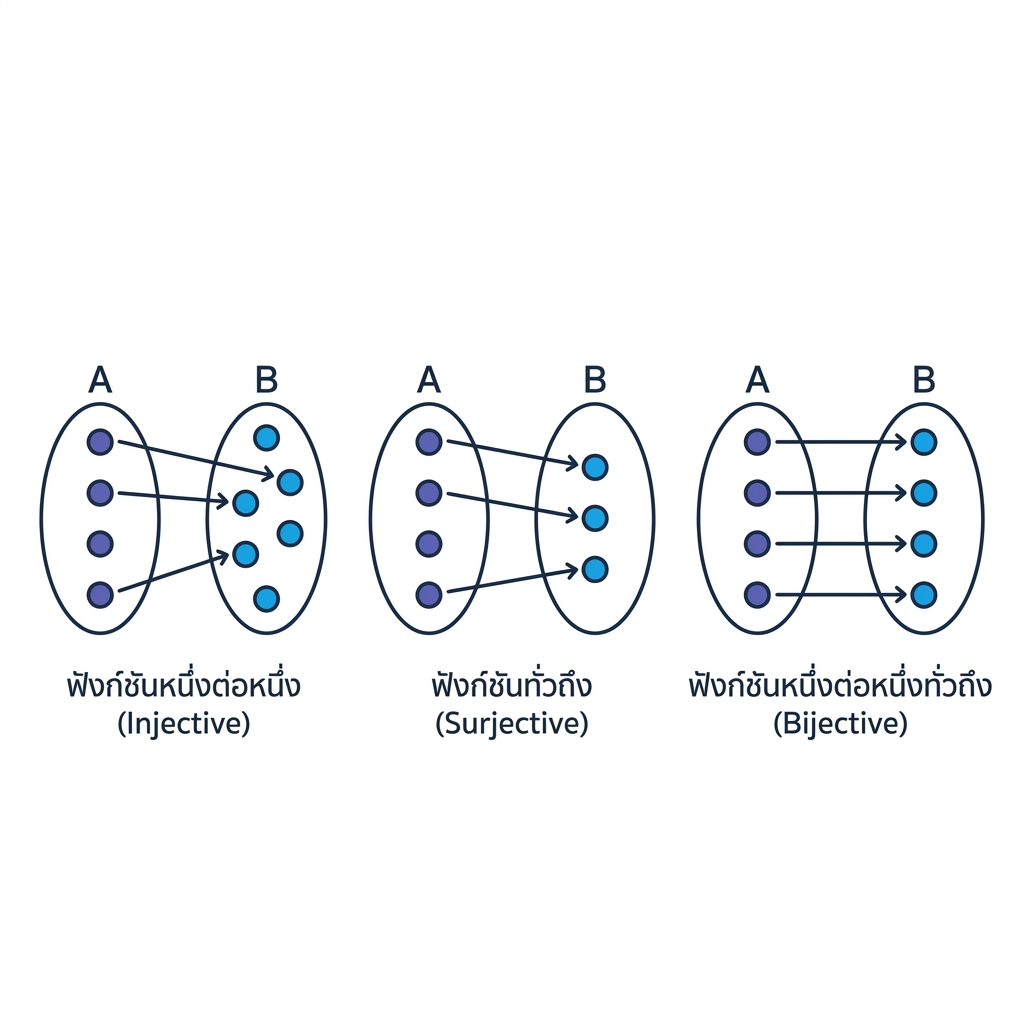
\includegraphics[width=0.68\textwidth]{Figures/png_ready/function-types-thai.png}
    \caption{แผนภาพเปรียบเทียบลักษณะการจับคู่ของฟังก์ชันหนึ่งต่อหนึ่ง ฟังก์ชันทั่วถึง และฟังก์ชันหนึ่งต่อหนึ่งทั่วถึง}
    \label{fig:function-types-thai}
\end{figure}

\begin{ex}
\label{ex:proof-bijective-real}
จงพิสูจน์ว่าฟังก์ชัน $f:\mathbb{R} \to \mathbb{R}$ ที่นิยามโดย $f(x) = x^3 + 1$ เป็นฟังก์ชันหนึ่งต่อหนึ่งทั่วถึง (Bijective)
\end{ex}
\begin{solution}
\begin{align*}
\text{หนึ่งต่อหนึ่ง} &\quad f(x_1) = f(x_2) \Rightarrow x_1^3 + 1 = x_2^3 + 1 \Rightarrow x_1^3 = x_2^3 \Rightarrow x_1 = x_2\\
\text{ทั่วถึง} &\quad \text{ให้ } y \in \mathbb{R},\ x^3 + 1 = y \Rightarrow x = \sqrt[3]{y - 1} \in \mathbb{R} \Rightarrow f(x) = y
\end{align*}
$\therefore f$ เป็นทั้งฟังก์ชันหนึ่งต่อหนึ่งและฟังก์ชันทั่วถึง จึงเป็นฟังก์ชันหนึ่งต่อหนึ่งทั่วถึง \solhere
\end{solution}

\subsection{การประกอบฟังก์ชันและฟังก์ชันผกผัน}
การคำนวณราคาสินค้าชำระเงินในระบบพาณิชย์อิเล็กทรอนิกส์ ประกอบด้วยขั้นตอนการคำนวณราคาสินค้าหลังหักส่วนลด ($f$) แล้วนำราคานั้นไปคำนวณภาษีมูลค่าเพิ่ม 7\% ต่อ ($g$) การทำงานต่อเนื่องสองขั้นตอนเรียกว่า การประกอบฟังก์ชัน ($g \circ f$) ขณะที่ฟังก์ชันผกผันคือกระบวนการคำนวณย้อนกลับจากยอดเงินสุทธิในใบเสร็จเพื่อหาว่าราคาสินค้าตั้งต้นก่อนหักส่วนลดมีค่าเท่าใด

\begin{definition}[การประกอบฟังก์ชัน และ ฟังก์ชันผกผัน]
\index{การประกอบฟังก์ชัน!นิยาม}
\index{ฟังก์ชันผกผัน!นิยาม}
\begin{enumerate}[label=\textbf{\arabic*.}]
    \item การประกอบฟังก์ชัน $g \circ f$ สำหรับ $f:A \to B$ และ $g:B \to C$ นิยามโดย $(g \circ f)(a) = g(f(a))$
    \item ฟังก์ชันผกผัน $f^{-1}$ ของฟังก์ชันหนึ่งต่อหนึ่งทั่วถึง $f:A \to B$ คือฟังก์ชัน $f^{-1}:B \to A$ ซึ่ง $f^{-1}(b) = a \iff f(a) = b$
\end{enumerate}
\end{definition}

การประกอบฟังก์ชันเกิดขึ้นได้ก็ต่อเมื่อเรนจ์ของฟังก์ชันที่ทำก่อนอยู่ภายในโดเมนของฟังก์ชันที่ทำทีหลัง ผลลัพธ์ที่ได้จึงเป็นฟังก์ชันใหม่ที่รับข้อมูลจากเซต $A$ แล้วส่งออกไปยังเซต $C$ โดยตรง โดยมีเซต $B$ ทำหน้าที่เป็นสถานะกลางที่ผู้ใช้งานไม่จำเป็นต้องรับรู้ ดังแสดงใน~\autoref{fig:function-composition}

\begin{figure}[H]
    \centering
    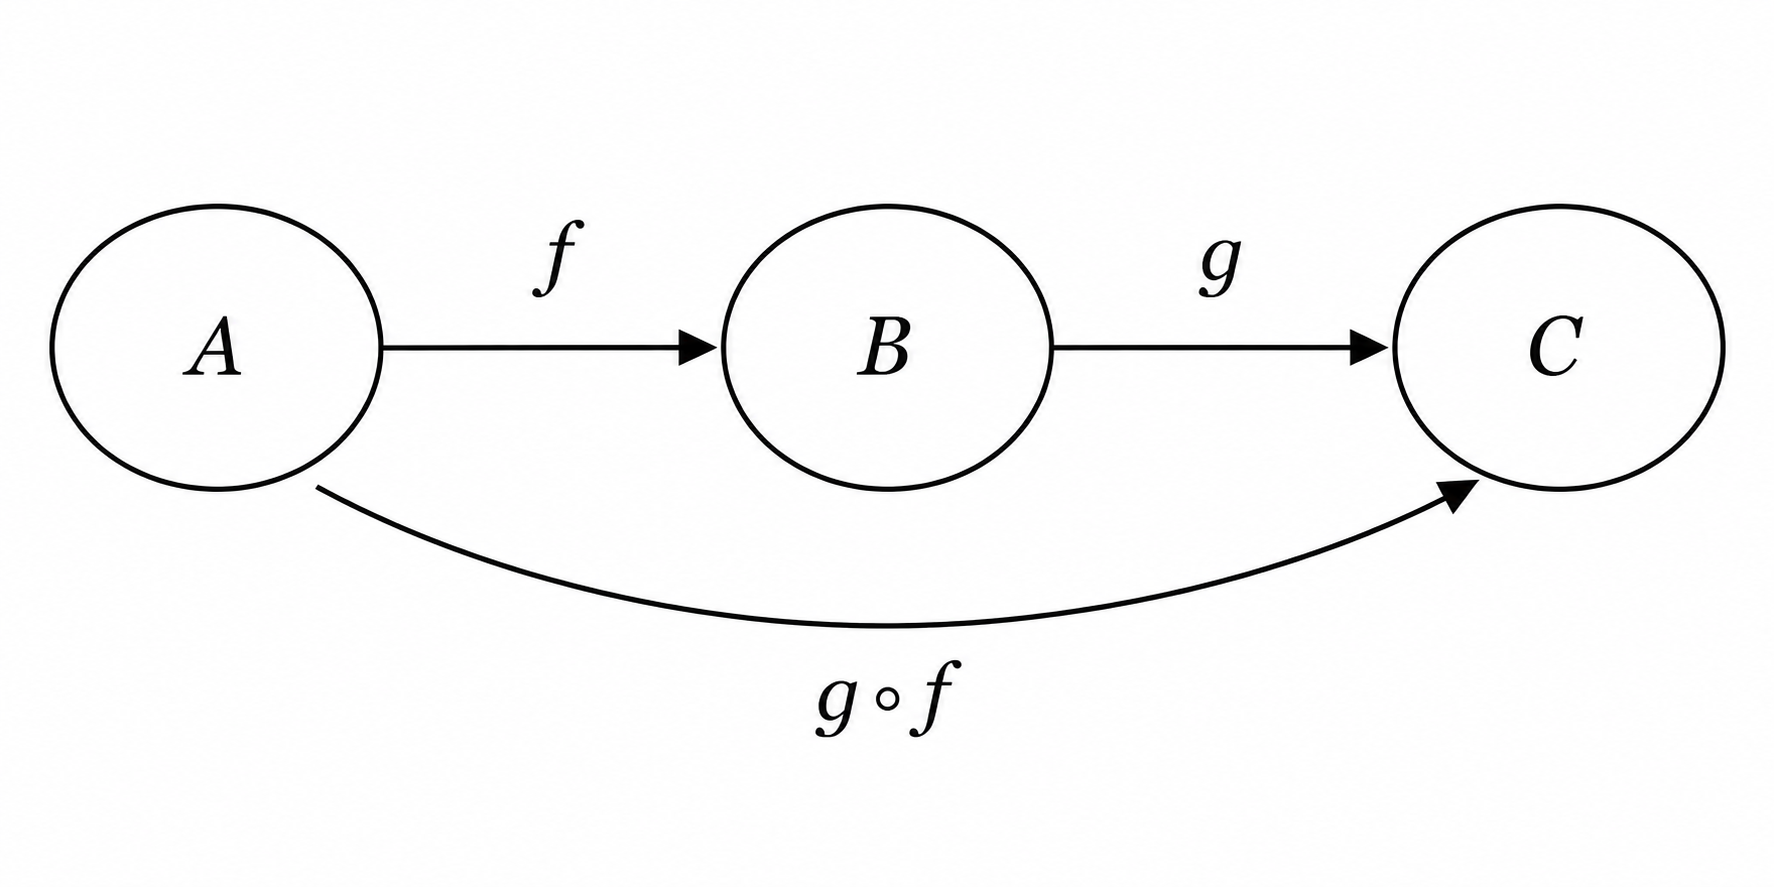
\includegraphics[width=0.62\textwidth]{Figures/png_ready/37-function-composition-manual.png}
    \caption{แผนภาพแสดงการประกอบฟังก์ชัน $(g \circ f)(a) = g(f(a))$ ที่ส่งผ่านข้อมูลจากเซต $A$ ผ่าน $B$ ไปยัง $C$}
    \label{fig:function-composition}
\end{figure}

\begin{ex}
ให้ $f(x)=2x+1$ บน $\mathbb{R}$ จงหา $(f \circ f)(x)$ และ $f^{-1}(x)$
\end{ex}
\begin{solution}
\begin{align*}
(f \circ f)(x) &= f(f(x)) = f(2x+1) = 2(2x+1)+1 = 4x+3\\
y = 2x+1 &\Rightarrow x = \frac{y-1}{2} \Rightarrow f^{-1}(x) = \frac{x-1}{2}
\end{align*}
$\therefore (f \circ f)(x) = 4x+3$ และ $f^{-1}(x) = \dfrac{x-1}{2}$ \solhere
\end{solution}

\begin{ex}
\label{ex:composition-inverse-two-func}
กำหนดฟังก์ชัน $f(x) = 3x - 4$ และ $g(x) = 2x + 5$ บน $\mathbb{R}$ จงหา $(g \circ f)(x)$ และ $(g \circ f)^{-1}(x)$
\end{ex}
\begin{solution}
\begin{align*}
(g \circ f)(x) &= g(f(x)) = g(3x-4) = 2(3x-4) + 5 = 6x - 8 + 5 = 6x - 3\\
y = 6x - 3 &\Rightarrow 6x = y + 3 \Rightarrow x = \frac{y+3}{6} \Rightarrow (g \circ f)^{-1}(x) = \frac{x+3}{6}
\end{align*}
$\therefore (g \circ f)(x) = 6x - 3$ และ $(g \circ f)^{-1}(x) = \dfrac{x+3}{6}$ \solhere
\end{solution}

\subsection{ฟังก์ชันพิเศษในทางคอมพิวเตอร์}
การประมวลผลข้อมูลในระบบคอมพิวเตอร์อาศัยการคำนวณรูปแบบเฉพาะ เช่น การจัดสรรยานพาหนะขนส่งผู้โดยสาร 45 คน โดยรถบัส 1 คันรองรับได้ 10 คน ระบบต้องปัดเศษขึ้นเป็น 5 คัน ($\lceil 45/10 \rceil = 5$) หรือการจัดลำดับการทำงานวนซ้ำทุก 7 วัน การดำเนินงานลักษณะนี้สอดคล้องกับฟังก์ชันพิเศษ ได้แก่ ฟังก์ชันปัดลง (Floor) ฟังก์ชันปัดขึ้น (Ceiling) และฟังก์ชันมอดูโล (Modulo)

\begin{definition}[ฟังก์ชันพิเศษ]
\index{ฟังก์ชันพิเศษ!Floor and Ceiling}
\index{ฟังก์ชันพิเศษ!Hash Function}
\begin{enumerate}[label=\textbf{\arabic*.}]
    \item ฟังก์ชันปัดลง (Floor) เขียนแทนด้วย $\lfloor x \rfloor$ คือจำนวนเต็มที่มากที่สุดซึ่งมีค่าน้อยกว่าหรือเท่ากับ $x$
    \item ฟังก์ชันปัดขึ้น (Ceiling) เขียนแทนด้วย $\lceil x \rceil$ คือจำนวนเต็มที่น้อยที่สุดซึ่งมีค่ามากกว่าหรือเท่ากับ $x$
    \item ฟังก์ชันมอดูโล (Modulo) เขียนแทนด้วย $x \bmod m$ คือเศษเหลือ $r$ ที่ทำให้ $x = qm + r$ โดยที่ $q \in \mathbb{Z}$ และ $0 \le r < m$ เมื่อ $m > 0$
    \item ฟังก์ชันแฮช (Hash Function) คือฟังก์ชัน $h: K \to S$ ที่แปลงคีย์ข้อมูลเป็นดรรชนีตำแหน่งจัดเก็บ เช่น $h(k) = k \bmod m$
\end{enumerate}
\end{definition}

นิยามของฟังก์ชันมอดูโลข้างต้นบังคับให้เศษเหลืออยู่ในช่วง $0 \le r < m$ เสมอ ผลลัพธ์ของตัวตั้งที่เป็นจำนวนลบจึงยังคงเป็นจำนวนไม่ติดลบ เช่น $-15 \bmod 4 = 1$ ข้อควรระวังในทางปฏิบัติคือภาษาโปรแกรมไม่ได้ใช้นิยามนี้ทั้งหมด ภาษา Python และ Ruby ให้ผลลัพธ์ตรงกับนิยามทางคณิตศาสตร์ ขณะที่ภาษา C, C++, Java และ JavaScript ใช้การหารแบบตัดเศษเข้าหาศูนย์ ทำให้ตัวดำเนินการ \texttt{\%} คืนค่า $-3$ สำหรับนิพจน์เดียวกัน ผู้เขียนโปรแกรมที่ต้องการผลลัพธ์ไม่ติดลบในภาษากลุ่มหลังจึงต้องเขียนเป็น \texttt{((x \% m) + m) \% m}

\begin{ex}
\label{ex:special-functions-calc}
จงคำนวณค่าของฟังก์ชันพิเศษต่อไปนี้
\begin{enumerate}[label=\textbf{\arabic*.}]
    \item $\lfloor 3.8 \rfloor$ และ $\lfloor -2.3 \rfloor$
    \item $\lceil 3.1 \rceil$ และ $\lceil -2.8 \rceil$
    \item $27 \bmod 6$ และ $-15 \bmod 4$
    \item ค่าแฮช $h(108)$ สำหรับฟังก์ชันแฮช $h(k) = k \bmod 11$
\end{enumerate}
\end{ex}
\begin{solution}
\begin{align*}
\lfloor 3.8 \rfloor &= 3, \qquad \lfloor -2.3 \rfloor = -3\\
\lceil 3.1 \rceil &= 4, \qquad \lceil -2.8 \rceil = -2\\
27 \bmod 6 &= 3 \quad (27 = 4 \times 6 + 3)\\
-15 \bmod 4 &= 1 \quad (-15 = -4 \times 4 + 1)\\
h(108) &= 108 \bmod 11 = 9 \quad (108 = 9 \times 11 + 9)
\end{align*}
\solhere
\end{solution}

\section{ลำดับและอนุกรม (Sequences and Series)}
\label{sec:sequences-and-series}

ในทางคณิตศาสตร์และคอมพิวเตอร์ ลำดับ (Sequence) คือฟังก์ชันที่มีโดเมนเป็นเซตของจำนวนเต็มบวก $\mathbb{Z}^+$ เขียนแทนด้วย $a: \mathbb{Z}^+ \to S$ หรือ $a_n = a(n)$ และเมื่อนำพจน์ในลำดับมาบวกสะสมกันจะเรียกว่า อนุกรม (Series) ซึ่งสอดคล้องกับพฤติกรรมการทำงานของวนลูป (Loop) และการวิเคราะห์ประสิทธิภาพของอัลกอริทึม

\subsection{ลำดับเลขคณิต (Arithmetic Sequence)}
พิจารณาการออมเงินโดยเริ่มต้นฝากเงินวันแรก 10 บาท และเพิ่มเงินฝากขึ้นวันละ 5 บาทอย่างสม่ำเสมอ จำนวนเงินฝากในแต่ละวันจะเป็น 10, 15, 20, 25,... ซึ่งเรียงลำดับเป็นลำดับเลขคณิต การคำนวณเงินฝาก ณ วันที่ 30 คือการหาพจน์ของลำดับ ส่วนการคำนวณเงินออมสะสมรวมทั้งหมดตั้งแต่วันแรกถึงวันที่ 30 คือการคำนวณผลรวมอนุกรมเลขคณิต

\begin{definition}[ลำดับเลขคณิต]
\index{ลำดับ!เลขคณิต}
ลำดับเลขคณิต (Arithmetic Sequence) คือลำดับที่ผลต่างของพจน์ที่อยู่ติดกันมีค่าคงตัว เรียกว่า ผลต่างร่วม (Common Difference) เขียนแทนด้วย $d = a_{n+1} - a_n$ โดยมีพจน์ทั่วไป (General Term) นิยามโดย
\[ a_n = a_1 + (n-1)d \]
เมื่อ $a_1$ คือพจน์แรก และ $n$ คือลำดับพจน์ที่ต้องการคำนวณ
\end{definition}

\begin{ex}
กำหนดลำดับเลขคณิต $3, 7, 11, 15, \dots$ จงหาผลต่างร่วม $d$ และพจน์ที่ 20 ($a_{20}$)
\end{ex}
\begin{solution}
\begin{align*}
a_1 &= 3, \quad d = 7 - 3 = 4\\
a_{20} &= a_1 + (20-1)d = 3 + (19)(4) = 3 + 76 = 79
\end{align*}
$\therefore d = 4$ และ $a_{20} = 79$ \solhere
\end{solution}

\begin{ex}
\label{ex:arithmetic-sequence-find-n}
กำหนดลำดับเลขคณิต $7, 11, 15, 19, \dots, 83$ จงหาว่าลำดับนี้มีทั้งหมดกี่พจน์
\end{ex}
\begin{solution}
\begin{align*}
a_1 &= 7, \quad d = 11 - 7 = 4, \quad a_n = 83\\
83 &= 7 + (n-1)4\\
76 &= (n-1)4\\
n - 1 &= 19 \ \Rightarrow \ n = 20
\end{align*}
$\therefore$ ลำดับนี้มีทั้งหมด 20 พจน์ \solhere
\end{solution}

\subsection{ลำดับเรขาคณิต (Geometric Sequence)}
พิจารณาการแพร่กระจายข้อมูลในเครือข่ายสังคม หากบุคคล 1 คนส่งต่อข้อมูลให้ผู้รับ 2 คน จากนั้นผู้รับทั้ง 2 คนนำไปส่งต่อให้ผู้รับรายใหม่คนละ 2 คน จำนวนผู้รับข้อมูลจะเพิ่มขึ้นเป็น 4, 8, 16 คนตามลำดับ การเพิ่มขึ้นในลักษณะทวีคูณนี้คือ ลำดับเรขาคณิต และการคำนวณจำนวนผู้ได้รับข้อมูลทั้งหมดในระบบคือ อนุกรมเรขาคณิต

\begin{definition}[ลำดับเรขาคณิต]
\index{ลำดับ!เรขาคณิต}
ลำดับเรขาคณิต (Geometric Sequence) คือลำดับที่อัตราส่วนของพจน์ที่อยู่ติดกันมีค่าคงตัว เรียกว่า อัตราส่วนร่วม (Common Ratio) เขียนแทนด้วย $r = \frac{a_{n+1}}{a_n}$ โดยมีพจน์ทั่วไปนิยามโดย
\[ a_n = a_1 r^{n-1} \]
เมื่อ $a_1$ คือพจน์แรก และ $r \neq 0$ คืออัตราส่วนร่วม
\end{definition}

\begin{ex}
กำหนดลำดับเรขาคณิต $2, 6, 18, 54, \dots$ จงหาอัตราส่วนร่วม $r$ และพจน์ที่ 7 ($a_7$)
\end{ex}
\begin{solution}
\begin{align*}
a_1 &= 2, \quad r = \frac{6}{2} = 3\\
a_7 &= a_1 r^{7-1} = 2 \times 3^6 = 2 \times 729 = 1458
\end{align*}
$\therefore r = 3$ และ $a_7 = 1458$ \solhere
\end{solution}

\subsection{อนุกรมเลขคณิต (Arithmetic Series)}
การหาผลรวมสะสมของข้อมูลในลำดับเลขคณิตตั้งแต่พจน์แรกจนถึงพจน์ที่ต้องการ เรียกว่า อนุกรมเลขคณิต ในทางคอมพิวเตอร์ การคำนวณผลรวมนี้สอดคล้องกับการหาจำนวนรอบการทำงานรวมของวนลูปซ้อน (Nested Loop) ที่มีจำนวนรอบเปลี่ยนไปอย่างเป็นรูปธรรม

\begin{definition}[อนุกรมเลขคณิต]
\index{อนุกรม!เลขคณิต}
อนุกรมเลขคณิต (Arithmetic Series) คือผลรวมของพจน์ในลำดับเลขคณิต เขียนแทนด้วย $S_n = \sum_{i=1}^{n} a_i$ โดยมีสูตรคำนวณผลรวม $n$ พจน์แรกดังนี้
\[ S_n = \frac{n(a_1 + a_n)}{2} = \frac{n[2a_1 + (n-1)d]}{2} \]
\end{definition}

\begin{ex}
จงหาผลรวม 10 พจน์แรก ($S_{10}$) ของอนุกรมเลขคณิต $5 + 8 + 11 + 14 + \dots$
\end{ex}
\begin{solution}
\begin{align*}
a_1 &= 5, \quad d = 8 - 5 = 3, \quad n = 10\\
S_{10} &= \frac{n[2a_1 + (n-1)d]}{2} = \frac{10[2(5) + 9(3)]}{2}\\
&= 5[10 + 27] = 5 \times 37 = 185
\end{align*}
$\therefore$ ผลรวม 10 พจน์แรก $S_{10} = 185$ \solhere
\end{solution}

\subsection{อนุกรมเรขาคณิต (Geometric Series)}
ในการวิเคราะห์ประสิทธิภาพของอัลกอริทึมแบบแบ่งแยกและเอาชนะ (Divide and Conquer) ผลรวมของภาระงานในทุกระดับชั้นของโครงสร้างการประมวลผลสามารถเขียนแทนได้ด้วยอนุกรมเรขาคณิต สูตรคำนวณผลรวมอนุกรมเรขาคณิตจึงช่วยให้ประเมินขอบเขตเวลาการทำงานรวมของโปรแกรมได้อย่างรวดเร็ว

\begin{definition}[อนุกรมเรขาคณิต]
\index{อนุกรม!เรขาคณิต}
อนุกรมเรขาคณิต (Geometric Series) คือผลรวมของพจน์ในลำดับเรขาคณิต เขียนแทนด้วย $S_n = \sum_{i=1}^{n} a_1 r^{i-1}$ โดยมีสูตรคำนวณผลรวม $n$ พจน์แรกดังนี้
\[ S_n = \frac{a_1(r^n - 1)}{r - 1} = \frac{a_1(1 - r^n)}{1 - r} \quad (\text{เมื่อ } r \neq 1) \qquad S_n = n a_1 \quad (\text{เมื่อ } r = 1) \]
และเมื่อ $\lvert r \rvert < 1$ ผลรวมของพจน์ทั้งหมดอย่างไม่จำกัดจำนวนจะลู่เข้าสู่ค่าจำกัด เรียกว่าผลรวมอนันต์ (Infinite Sum) นิยามโดย
\[ S_\infty = \sum_{i=1}^{\infty} a_1 r^{i-1} = \frac{a_1}{1 - r} \]
\end{definition}

สูตรทั้งสองรูปของ $S_n$ เมื่อ $r \neq 1$ มีค่าเท่ากันเสมอ เพราะเกิดจากการคูณทั้งเศษและส่วนด้วย $-1$ การเลือกใช้รูปใดจึงเป็นเพียงความสะดวกในการคำนวณ โดยนิยมใช้รูปแรกเมื่อ $r > 1$ เพื่อให้ตัวส่วนเป็นบวก และใช้รูปที่สองเมื่อ $r < 1$ ด้วยเหตุผลเดียวกัน ส่วนกรณี $r = 1$ ต้องแยกพิจารณาต่างหาก เนื่องจากตัวส่วน $r - 1$ มีค่าเป็นศูนย์ ซึ่งในกรณีนี้ทุกพจน์มีค่าเท่ากับ $a_1$ ผลรวมจึงเท่ากับ $n a_1$

\begin{ex}
จงหาผลรวม 6 พจน์แรก ($S_6$) ของอนุกรมเรขาคณิต $3 + 6 + 12 + 24 + \dots$
\end{ex}
\begin{solution}
\begin{align*}
a_1 &= 3, \quad r = \frac{6}{3} = 2, \quad n = 6\\
S_6 &= \frac{a_1(r^n - 1)}{r - 1} = \frac{3(2^6 - 1)}{2 - 1} = \frac{3(64-1)}{1} = 3 \times 63 = 189
\end{align*}
$\therefore$ ผลรวม 6 พจน์แรก $S_6 = 189$ \solhere
\end{solution}

\begin{ex}
\label{ex:infinite-geometric-series}
จงหาผลรวมอนันต์ ($S_\infty$) ของอนุกรมเรขาคณิต $12 + 6 + 3 + 1.5 + \dots$
\end{ex}
\begin{solution}
\begin{align*}
a_1 &= 12, \quad r = \frac{6}{12} = \frac{1}{2} \quad (\lvert r \rvert < 1 \text{ อนุกรมจึงลู่เข้า})\\
S_\infty &= \frac{a_1}{1 - r} = \frac{12}{1 - \tfrac{1}{2}} = \frac{12}{\tfrac{1}{2}} = 24
\end{align*}
$\therefore$ ผลรวมอนันต์ $S_\infty = 24$ \solhere
\end{solution}

\section{การประยุกต์ใช้ในวิทยาการคอมพิวเตอร์}
\label{sec:relation-applications}

แนวคิดเรื่องความสัมพันธ์ ฟังก์ชัน ลำดับ และอนุกรม ถูกนำไปใช้เป็นแกนหลักในการออกแบบซอฟต์แวร์และโครงสร้างข้อมูลทางคอมพิวเตอร์ หัวข้อนี้ยกตัวอย่างการประยุกต์ใช้ในสามบริบทที่นักศึกษาจะพบในรายวิชาถัดไป ได้แก่ การจัดเก็บข้อมูลเชิงตารางในระบบฐานข้อมูล การกำหนดลำดับการทำงานของคำสั่งในตัวแปลภาษา และการจัดสรรตำแหน่งจัดเก็บข้อมูลในตารางแฮช ทั้งสามบริบทอาศัยแนวคิดเดียวกันคือการมองการจับคู่ระหว่างข้อมูลเป็นเซตของคู่อันดับที่มีสมบัติทางคณิตศาสตร์กำกับ

\subsection{ฐานข้อมูลเชิงสัมพันธ์และพีชคณิตเชิงสัมพันธ์}
แบบจำลองฐานข้อมูลเชิงสัมพันธ์ (Relational Model) ที่เอ็ดการ์ คอดด์ เสนอไว้ในปี ค.ศ. 1970 มองตารางข้อมูลหนึ่งตารางเป็นความสัมพันธ์ทางคณิตศาสตร์ $R \subseteq A_1 \times A_2 \times \dots \times A_n$ เมื่อ $A_i$ คือเซตของค่าที่คอลัมน์ที่ $i$ รับได้~\cite{codd1970relational} แต่ละแถวของตารางคือทูเปิล (Tuple) ซึ่งก็คือสมาชิกหนึ่งตัวของความสัมพันธ์ ส่วนแต่ละคอลัมน์คือแอตทริบิวต์ (Attribute) ซึ่งกำหนดความหมายของค่าในตำแหน่งนั้น การมองตารางเป็นเซตทำให้การสืบค้นข้อมูลกลายเป็นการดำเนินการบนเซตที่มีนิยามทางคณิตศาสตร์รองรับ เรียกว่าพีชคณิตเชิงสัมพันธ์ (Relational Algebra)

การดำเนินการพื้นฐานของพีชคณิตเชิงสัมพันธ์สอดคล้องโดยตรงกับการดำเนินการบนเซตที่ศึกษามาแล้ว การเลือก (Selection) เขียนแทนด้วย $\sigma_{\varphi}(R)$ คือการคัดเฉพาะทูเปิลที่ทำให้เงื่อนไข $\varphi$ เป็นจริง ซึ่งก็คือการสร้างเซตย่อยของ $R$ การฉาย (Projection) เขียนแทนด้วย $\pi_{A_i}(R)$ คือการเลือกเฉพาะบางแอตทริบิวต์ ซึ่งให้ผลเป็นเรนจ์ของความสัมพันธ์เมื่อพิจารณาเฉพาะคอลัมน์ที่สนใจ และการเชื่อมตามธรรมชาติ (Natural Join) เขียนแทนด้วย $R \bowtie S$ คือการจับคู่ทูเปิลจากสองตารางที่มีค่าตรงกันในแอตทริบิวต์ร่วม ซึ่งเป็นรูปแบบหนึ่งของการประกอบความสัมพันธ์ที่ศึกษาใน~\autoref{sec:relation-properties}

\subsection{การจัดลำดับการทำงานของโปรแกรม}
ในตัวแปลภาษา การวิเคราะห์ไวยากรณ์ (Parsing) ต้องตรวจสอบว่าวงเล็บเปิดและวงเล็บปิดในนิพจน์จับคู่กันครบถ้วนหรือไม่ กระบวนการนี้อาศัยฟังก์ชันที่ส่งนิพจน์ไปยังค่าความจริงว่าสมดุลหรือไม่สมดุล โดยใช้โครงสร้างข้อมูลกองซ้อน (Stack) เก็บวงเล็บเปิดที่ยังไม่ถูกจับคู่ นิพจน์จะสมดุลก็ต่อเมื่ออ่านจนจบแล้วกองซ้อนว่างเปล่าพอดี

การจัดลำดับการทำงานของคำสั่งที่ต้องประมวลผลตามลำดับก่อนหลังใช้ความสัมพันธ์ $R = \{(s_1, s_2) \mid s_1 \text{ ต้องทำงานเสร็จก่อน } s_2\}$ ซึ่งต้องมีคุณสมบัติปฏิสมมาตรและถ่ายทอด หากความสัมพันธ์นี้เกิดวงจรปิด เช่น คำสั่ง $s_1$ ต้องรอ $s_2$ ขณะที่ $s_2$ ก็ต้องรอ $s_1$ ระบบจะเข้าสู่ภาวะติดตาย (Deadlock) และไม่มีคำสั่งใดทำงานต่อได้ การตรวจสอบว่าความสัมพันธ์ปลอดวงจรปิดจึงทำได้โดยคำนวณการปิดถ่ายทอด $t(R)$ แล้วตรวจว่ามีคู่อันดับในรูป $(s,s)$ ปรากฏขึ้นหรือไม่

\subsection{การจัดเก็บข้อมูลด้วยตารางแฮชและการแก้ปัญหาการชนกัน}
ตารางแฮช (Hash Table) ใช้ฟังก์ชันแฮชแปลงคีย์ข้อมูลให้เป็นดรรชนีตำแหน่งจัดเก็บโดยตรง จึงเข้าถึงข้อมูลได้โดยไม่ต้องค้นหาทีละตำแหน่ง อย่างไรก็ตาม ฟังก์ชันแฮชโดยทั่วไปไม่ใช่ฟังก์ชันหนึ่งต่อหนึ่ง เพราะจำนวนคีย์ที่เป็นไปได้มักมากกว่าจำนวนช่องในตาราง เมื่อคีย์ต่างกันสองตัวถูกส่งไปยังดรรชนีเดียวกันจะเรียกว่าการชนกัน (Collision) วิธีแก้ปัญหาที่ตรงไปตรงมาที่สุดคือการสำรวจเชิงเส้น (Linear Probing) ซึ่งเลื่อนไปตรวจช่องถัดไปทีละหนึ่งตำแหน่งจนกว่าจะพบช่องว่าง

\begin{ex}
\label{ex:hash-table-linear-probing}
กำหนดฟังก์ชันแฮช $h(k) = k \bmod 7$ และชุดคีย์ $K = \{12, 19, 26, 33\}$ จงหาดรรชนีแฮช และแสดงการจัดเก็บข้อมูลด้วย Linear Probing เมื่อเกิดการชนกัน
\end{ex}
\begin{solution}
\begin{align*}
h(12) &= 12 \bmod 7 = 5 &&\Rightarrow \text{ช่องว่าง เก็บ } 12 \text{ ที่ดรรชนี } 5\\
h(19) &= 19 \bmod 7 = 5 &&\Rightarrow \text{ชนกัน}, \ (5+1) \bmod 7 = 6 \Rightarrow \text{เก็บ } 19 \text{ ที่ดรรชนี } 6\\
h(26) &= 26 \bmod 7 = 5 &&\Rightarrow \text{ชนกัน}, \ (5+2) \bmod 7 = 0 \Rightarrow \text{เก็บ } 26 \text{ ที่ดรรชนี } 0\\
h(33) &= 33 \bmod 7 = 5 &&\Rightarrow \text{ชนกัน}, \ (5+3) \bmod 7 = 1 \Rightarrow \text{เก็บ } 33 \text{ ที่ดรรชนี } 1
\end{align*}
$\therefore$ ตารางแฮชจัดเก็บข้อมูลที่ดรรชนี 0, 1, 5 และ 6 ด้วยคีย์ 26, 33, 12 และ 19 ตามลำดับ \solhere
\end{solution}

\sectionbanner{สรุปบทเรียน}
ความสัมพันธ์และฟังก์ชันเป็นรากฐานทางคณิตศาสตร์ที่สำคัญของโครงสร้างข้อมูลและการประมวลผลทางคอมพิวเตอร์ ความสัมพันธ์ $R \subseteq A \times B$ อธิบายการจับคู่ระหว่างสมาชิกสองเซต ความสัมพันธ์ทวิภาคบนเซตเดียวกันจำแนกตามคุณสมบัติสะท้อน สมมาตร ปฏิสมมาตร และถ่ายทอด รวมถึงการปิดคุณสมบัติสะท้อน สมมาตร และถ่ายทอดเพื่อวิเคราะห์การเชื่อมต่อในทฤษฎีกราฟ

ฟังก์ชัน $f: A \to B$ จัดเป็นความสัมพันธ์ชนิดพิเศษที่สมาชิกต้นทางทุกตัวถูกจับคู่ไปยังสมาชิกปลายทางเพียงตัวเดียว จำแนกเป็นฟังก์ชันหนึ่งต่อหนึ่ง ทั่วถึง และหนึ่งต่อหนึ่งทั่วถึง ซึ่งรองรับการประกอบฟังก์ชัน $(g \circ f)$ ฟังก์ชันผกผัน $f^{-1}$ รวมถึงฟังก์ชันพิเศษในทางคอมพิวเตอร์ ได้แก่ ฟังก์ชันปัดลง ฟังก์ชันปัดขึ้น ฟังก์ชันมอดูโล และฟังก์ชันแฮช

นอกจากนี้ การศึกษายังครอบคลุมถึงลำดับและอนุกรม ได้แก่ ลำดับเลขคณิต ($a_n = a_1 + (n-1)d$), ลำดับเรขาคณิต ($a_n = a_1 r^{n-1}$), อนุกรมเลขคณิต ($S_n = \frac{n(a_1+a_n)}{2}$) และอนุกรมเรขาคณิต ($S_n = \frac{a_1(r^n-1)}{r-1}$) ซึ่งเป็นแกนหลักของการคำนวณแบบวนลูปและการวิเคราะห์ประสิทธิภาพอัลกอริทึม ทั้งหมดนี้ได้รับการประยุกต์ใช้ในระบบฐานข้อมูลเชิงสัมพันธ์ การตรวจสอบไวยากรณ์คอมไพเลอร์ และการจัดลำดับการทำงานขนาน

\clearpage
\sectionbanner{แบบฝึกหัด}

\exercisepart{ส่วนที่ 1: ความสัมพันธ์และคู่อันดับ}
\begin{exercise}
กำหนดให้ $A = \{1, 2, 3\}$ และ $B = \{a, b\}$ จงหาสิ่งต่อไปนี้
\begin{enumerate}
    \item $A \times B$ และ $B \times A$
    \item จำนวนความสัมพันธ์ทั้งหมดที่เป็นไปได้จาก $A$ ไป $B$
    \item จำนวนความสัมพันธ์ทวิภาคทั้งหมดบนเซต $A$
\end{enumerate}
\end{exercise}

\begin{exercise}
กำหนด $A = \{1, 2, 3, 4\}$ และความสัมพันธ์ $R = \{(x,y) \in A \times A \mid x + y \le 5\}$ จงหาสิ่งต่อไปนี้
\begin{enumerate}
    \item สมาชิกทั้งหมดในความสัมพันธ์ $R$
    \item โดเมน $\mathcal{D}(R)$ และเรนจ์ $\mathcal{R}(R)$
    \item ความสัมพันธ์ผกผัน $R^{-1}$
\end{enumerate}
\end{exercise}

\exercisepart{ส่วนที่ 2: คุณสมบัติและการปิดคุณสมบัติของความสัมพันธ์}
\begin{exercise}
พิจารณาความสัมพันธ์ทวิภาคต่อไปนี้บนเซต $A = \{1, 2, 3, 4\}$ ว่ามีคุณสมบัติ สะท้อน, สมมาตร, ปฏิสมมาตร, หรือถ่ายทอด หรือไม่
\begin{enumerate}
    \item $R_1 = \{(1,1), (2,2), (3,3), (4,4)\}$
    \item $R_2 = \{(1,2), (2,1), (2,3), (3,2)\}$
    \item $R_3 = \{(1,1), (1,2), (2,2), (2,3), (1,3)\}$
    \item $R_4 = \{(1,2), (3,4)\}$
\end{enumerate}
\end{exercise}

\begin{exercise}
กำหนด $A = \{1, 2, 3\}$ และความสัมพันธ์ $R = \{(1,2), (2,3)\}$ จงหาสิ่งต่อไปนี้
\begin{enumerate}
    \item การปิดสะท้อน (Reflexive Closure) $r(R)$
    \item การปิดสมมาตร (Symmetric Closure) $s(R)$
    \item การปิดถ่ายทอด (Transitive Closure) $t(R)$
\end{enumerate}
\end{exercise}

\exercisepart{ส่วนที่ 3: นิยามและประเภทของฟังก์ชัน}
\begin{exercise}
พิจารณาว่าความสัมพันธ์ต่อไปนี้เป็นฟังก์ชันจาก $A = \{1, 2, 3\}$ ไปยัง $B = \{a, b, c\}$ หรือไม่ พร้อมระบุประเภทของฟังก์ชัน
\begin{enumerate}
    \item $f_1 = \{(1,a), (2,b), (3,c)\}$
    \item $f_2 = \{(1,a), (2,a), (3,b)\}$
    \item $f_3 = \{(1,a), (1,b), (2,c), (3,a)\}$
    \item $f_4 = \{(1,b), (2,c), (3,a)\}$
\end{enumerate}
\end{exercise}

\begin{exercise}
กำหนดฟังก์ชัน $f(x) = 3x - 5$ บนเซตของจำนวนจริง $\mathbb{R}$
\begin{enumerate}
    \item จงพิสูจน์ว่า $f$ เป็นฟังก์ชันหนึ่งต่อหนึ่ง (Injective)
    \item จงพิสูจน์ว่า $f$ เป็นฟังก์ชันทั่วถึง (Surjective)
    \item จงหาฟังก์ชันผกผัน $f^{-1}(x)$
\end{enumerate}
\end{exercise}

\exercisepart{ส่วนที่ 4: การประกอบฟังก์ชันและฟังก์ชันพิเศษ}
\begin{exercise}
กำหนด $f(x) = 2x + 3$ และ $g(x) = x^2 - 1$ บน $\mathbb{R}$ จงหาสิ่งต่อไปนี้
\begin{enumerate}
    \item $(g \circ f)(x)$ และ $(g \circ f)(2)$
    \item $(f \circ g)(x)$ และ $(f \circ g)(2)$
    \item $(f \circ f)(x)$
\end{enumerate}
\end{exercise}

\begin{exercise}
จงคำนวณค่าของฟังก์ชันพิเศษต่อไปนี้
\begin{enumerate}
    \item $\lfloor 4.8 \rfloor$ และ $\lfloor -3.2 \rfloor$
    \item $\lceil 2.1 \rceil$ และ $\lceil -1.7 \rceil$
    \item $37 \bmod 5$ และ $-14 \bmod 4$
    \item ค่าแฮช $h(k) = k \bmod 11$ เมื่อ $k = 125$
\end{enumerate}
\end{exercise}

\exercisepart{ส่วนที่ 5: ลำดับและอนุกรม}
\begin{exercise}
กำหนดลำดับเลขคณิต $4, 9, 14, 19, \dots$ จงหาสิ่งต่อไปนี้
\begin{enumerate}
    \item ผลต่างร่วม $d$ และพจน์ทั่วไป $a_n$
    \item พจน์ที่ 15 ($a_{15}$)
    \item ผลรวม 15 พจน์แรก ($S_{15}$)
\end{enumerate}
\end{exercise}

\begin{exercise}
กำหนดลำดับเรขาคณิต $3, 6, 12, 24, \dots$ จงหาสิ่งต่อไปนี้
\begin{enumerate}
    \item อัตราส่วนร่วม $r$ และพจน์ทั่วไป $a_n$
    \item พจน์ที่ 8 ($a_8$)
    \item ผลรวม 8 พจน์แรก ($S_8$)
\end{enumerate}
\end{exercise}

\answerkeyhead
\exercisepart{เฉลยส่วนที่ 1: ความสัมพันธ์และคู่อันดับ}
\begin{enumerate}[label={},leftmargin=0pt,itemsep=0.6em]
    \item
    \begin{enumerate}[label=\textbf{\thechapter.\arabic{enumi}.\arabic*}]
        \item $A \times B = \{(1,a),(1,b),(2,a),(2,b),(3,a),(3,b)\}$, $B \times A = \{(a,1),(a,2),(a,3),(b,1),(b,2),(b,3)\}$
        \item $2^{|A \times B|} = 2^6 = 64$ ความสัมพันธ์
        \item $2^{|A \times A|} = 2^9 = 512$ ความสัมพันธ์
    \end{enumerate}

    \item
    \begin{enumerate}[label=\textbf{\thechapter.\arabic{enumi}.\arabic*}]
        \item $R = \{(1,1),(1,2),(1,3),(1,4),(2,1),(2,2),(2,3),(3,1),(3,2),(4,1)\}$
        \item $\mathcal{D}(R) = \{1,2,3,4\}$, $\mathcal{R}(R) = \{1,2,3,4\}$
        \item $R^{-1} = \{(1,1),(2,1),(3,1),(4,1),(1,2),(2,2),(3,2),(1,3),(2,3),(1,4)\}$
    \end{enumerate}
\end{enumerate}

\exercisepart{เฉลยส่วนที่ 2: คุณสมบัติและการปิดคุณสมบัติของความสัมพันธ์}
\begin{enumerate}[label={},leftmargin=0pt,itemsep=0.6em]
    \setcounter{enumi}{2}
    \item
    \begin{enumerate}[label=\textbf{\thechapter.\arabic{enumi}.\arabic*}]
        \item $R_1$ เป็นสะท้อน สมมาตร ปฏิสมมาตร และถ่ายทอด ครบทั้งสี่ประการ
        \item $R_2$ เป็นสมมาตรเท่านั้น ไม่สะท้อน ไม่เป็นปฏิสมมาตร และไม่ถ่ายทอด
        \item $R_3$ เป็นปฏิสมมาตรและถ่ายทอด แต่ไม่สะท้อน เพราะขาด $(3,3)$ และ $(4,4)$
        \item $R_4$ เป็นปฏิสมมาตรและถ่ายทอด
    \end{enumerate}

    \item
    \begin{enumerate}[label=\textbf{\thechapter.\arabic{enumi}.\arabic*}]
        \item $r(R) = \{(1,1),(2,2),(3,3),(1,2),(2,3)\}$
        \item $s(R) = \{(1,2),(2,3),(2,1),(3,2)\}$
        \item $t(R) = \{(1,2),(2,3),(1,3)\}$
    \end{enumerate}
\end{enumerate}

\exercisepart{เฉลยส่วนที่ 3: นิยามและประเภทของฟังก์ชัน}
\begin{enumerate}[label={},leftmargin=0pt,itemsep=0.6em]
    \setcounter{enumi}{4}
    \item
    \begin{enumerate}[label=\textbf{\thechapter.\arabic{enumi}.\arabic*}]
        \item $f_1$ เป็นฟังก์ชันหนึ่งต่อหนึ่งทั่วถึง
        \item $f_2$ เป็นฟังก์ชัน แต่ไม่เป็นหนึ่งต่อหนึ่งและไม่เป็นทั่วถึง
        \item $f_3$ ไม่เป็นฟังก์ชัน เพราะสมาชิก 1 จับคู่ซ้ำทั้ง $a$ และ $b$
        \item $f_4$ เป็นฟังก์ชันหนึ่งต่อหนึ่งทั่วถึง
    \end{enumerate}

    \item
    \begin{enumerate}[label=\textbf{\thechapter.\arabic{enumi}.\arabic*}]
        \item ให้ $f(x_1) = f(x_2) \implies 3x_1 - 5 = 3x_2 - 5 \implies x_1 = x_2$ (เป็น Injective)
        \item ให้ $y \in \mathbb{R} \implies 3x - 5 = y \implies x = \frac{y+5}{3} \in \mathbb{R}$ (เป็น Surjective)
        \item $f^{-1}(x) = \dfrac{x+5}{3}$
    \end{enumerate}
\end{enumerate}

\exercisepart{เฉลยส่วนที่ 4: การประกอบฟังก์ชันและฟังก์ชันพิเศษ}
\begin{enumerate}[label={},leftmargin=0pt,itemsep=0.6em]
    \setcounter{enumi}{6}
    \item
    \begin{enumerate}[label=\textbf{\thechapter.\arabic{enumi}.\arabic*}]
        \item $(g \circ f)(x) = (2x+3)^2 - 1 = 4x^2 + 12x + 8$, $(g \circ f)(2) = 48$
        \item $(f \circ g)(x) = 2(x^2-1) + 3 = 2x^2 + 1$, $(f \circ g)(2) = 9$
        \item $(f \circ f)(x) = 4x + 9$
    \end{enumerate}

    \item
    \begin{enumerate}[label=\textbf{\thechapter.\arabic{enumi}.\arabic*}]
        \item $\lfloor 4.8 \rfloor = 4$, $\lfloor -3.2 \rfloor = -4$
        \item $\lceil 2.1 \rceil = 3$, $\lceil -1.7 \rceil = -1$
        \item $37 \bmod 5 = 2$, $-14 \bmod 4 = 2$
        \item $h(125) = 125 \bmod 11 = 4$
    \end{enumerate}
\end{enumerate}

\exercisepart{เฉลยส่วนที่ 5: ลำดับและอนุกรม}
\begin{enumerate}[label={},leftmargin=0pt,itemsep=0.6em]
    \setcounter{enumi}{8}
    \item
    \begin{enumerate}[label=\textbf{\thechapter.\arabic{enumi}.\arabic*}]
        \item $d = 5$, $a_n = 4 + (n-1)5 = 5n - 1$
        \item $a_{15} = 5(15) - 1 = 74$
        \item $S_{15} = \frac{15(4 + 74)}{2} = \frac{15(78)}{2} = 585$
    \end{enumerate}

    \item
    \begin{enumerate}[label=\textbf{\thechapter.\arabic{enumi}.\arabic*}]
        \item $r = 2$, $a_n = 3(2^{n-1})$
        \item $a_8 = 3(2^7) = 3(128) = 384$
        \item $S_8 = \frac{3(2^8 - 1)}{2 - 1} = 3(255) = 765$
    \end{enumerate}
\end{enumerate}

\newpage
\QAChapter
\begin{enumerate}
    \item จงอธิบายความแตกต่างระหว่างความสัมพันธ์ทั่วไปกับฟังก์ชัน ในมิติของการจับคู่ข้อมูลในระบบคอมพิวเตอร์
    \item เหตุใดคุณสมบัติสะท้อน (Reflexive) และคุณสมบัติสมมาตร (Symmetric) จึงมีความสำคัญในโครงสร้างกราฟและเครือข่ายคอมพิวเตอร์
    \item จงอธิบายการประยุกต์ใช้ฟังก์ชันแฮช (Hash Function) และการจัดการปัญหาการชนกันของข้อมูล (Collision) ในระบบฐานข้อมูล
    \item จงเปรียบเทียบลักษณะของฟังก์ชันหนึ่งต่อหนึ่ง (Injective) และฟังก์ชันทั่วถึง (Surjective) พร้อมยกตัวอย่างสถานการณ์ในงานคอมพิวเตอร์
    \item จงอธิบายการประกอบฟังก์ชัน $(g \circ f)(x)$ ในมุมมองของการประมวลผลท่อส่งข้อมูล (Data Pipeline) ในซอฟต์แวร์
    \item อธิบายความเชื่อมโยงระหว่างการปิดถ่ายทอด (Transitive Closure) กับอัลกอริทึมการหาเส้นทางเชื่อมต่อ (Path Reachability) ในทฤษฎีกราฟ
    \item จงอธิบายการนำลำดับเลขคณิตและลำดับเรขาคณิตไปใช้ในการคำนวณประสิทธิภาพและการจัดสรรทรัพยากรในระบบคอมพิวเตอร์
    \item จงอธิบายความเชื่อมโยงระหว่างอนุกรมและการผลรวมซิกมา ($\sum$) กับการคำนวณการวนลูป (Loop Complexity) ในภาษาโปรแกรม
\end{enumerate}

\newpage
\sheetChapter{ความสัมพันธ์และฟังก์ชัน (Relations and Functions)}
\section*{วัตถุประสงค์}
\begin{enumerate}
    \item เพื่อให้ผู้เรียนวิเคราะห์และระบุคุณสมบัติของความสัมพันธ์ทวิภาคและการปิดคุณสมบัติได้
    \item เพื่อให้ผู้เรียนจำแนกประเภทของฟังก์ชัน คำนวณการประกอบฟังก์ชัน และหาฟังก์ชันผกผันได้
    \item เพื่อให้ผู้เรียนคำนวณพจน์และผลรวมของลำดับเลขคณิต ลำดับเรขาคณิต อนุกรมเลขคณิต และอนุกรมเรขาคณิตได้
    \item เพื่อให้ผู้เรียนประยุกต์ใช้ความสัมพันธ์และฟังก์ชันในงานฐานข้อมูล ทฤษฎีกราฟ และตารางแฮชได้
\end{enumerate}
\section*{คำชี้แจง} ให้ผู้เรียนศึกษาเนื้อหาบทความสัมพันธ์และฟังก์ชัน แล้วตอบคำถามต่อไปนี้

\begin{enumerate}
    \item จงอธิบายความแตกต่างระหว่างความสัมพันธ์จาก $A$ ไป $B$ และฟังก์ชันจาก $A$ ไป $B$ พร้อมยกตัวอย่าง
    \Pointilles{3}
    \item กำหนด $A = \{1, 2, 3\}$ และ $R = \{(1,2), (2,3)\}$ จงหาการปิดสะท้อน $r(R)$, การปิดสมมาตร $s(R)$ และการปิดถ่ายทอด $t(R)$
    \Pointilles{3}
    \item กำหนด $f(x) = 4x - 7$ จงพิสูจน์ว่าเป็นฟังก์ชันหนึ่งต่อหนึ่งทั่วถึง และหา $f^{-1}(x)$
    \Pointilles{3}
    \item กำหนด $f(x) = 3x + 1$ และ $g(x) = x^2 + 2$ จงหา $(g \circ f)(x)$ และ $(f \circ g)(x)$
    \Pointilles{3}
    \item จงหาพจน์ที่ 10 ($a_{10}$) และผลรวม 10 พจน์แรก ($S_{10}$) ของลำดับเลขคณิต $2, 7, 12, 17, \dots$
    \Pointilles{3}
    \item จงอธิบายการนำทฤษฎีความสัมพันธ์และฟังก์ชันไปประยุกต์ใช้ในระบบฐานข้อมูล Relational Model หรือ Hash Table
    \Pointilles{3}
\end{enumerate}
